\chapter{Avaliação exploratória de soluções para o \textit{backend}}

\section{Cenário-tipo selecionado}

%explicar qual foi o cenário selecionado para experimentar em cada plataforma (deve ser uma parte dos requisitos gerais do capítulo 3)
Antes de avançar com o desenvolvimento do sistema foi necessário escolher um \textit{backend} para dar suporte tanto à aplicação móvel, como à aplicação \textit{web}. Para isso foi desenvolvido um cenário idêntico com os diferentes \textit{backends} em que pudéssemos fazer uma análise comparativa dos pontos fortes e ou fracos entre eles. \par 
O cenário escolhido para esta avaliação exploratória foi o simples ato de recolher a frequência cardíaca do sensor do \textit{VitalJacket} e guardar no \textit{backend} em estudo, para posteriormente ser possível a visualização de um histórico dos dados inseridos. Na figura \ref{f:study-overview} temos uma simples visão das várias partes envolvidas nesta avaliação exploratória.

\begin{figure}[H]
  \centering
  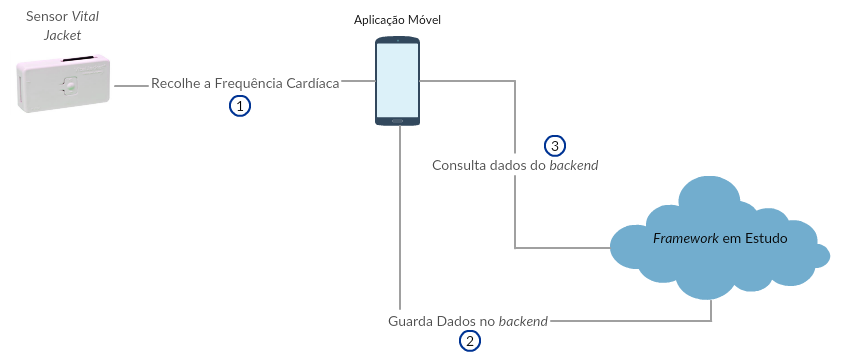
\includegraphics[width=0.9\textwidth]{imgs/study-overview.png}
  \caption[Diagrama geral do cenário de estudo]{Diagrama geral do cenário de estudo}
  
  \label{f:study-overview}
\end{figure}

A escolha de um \textit{backend} para a solução era um ponto importante. Das várias plataformas disponíveis para um possível \textit{backend} foram selecionadas três para ser desenvolvido o cenário com o objetivo de concluir se seria uma boa hipótese para a solução, entre elas estão: \gls{OMH}, \gls{FHIR} e \textit{Google Fit}. \par

Para utilizar cada uma destas plataformas, foi desenvolvida uma aplicação móvel, bastante simples. A aplicação móvel tinha várias funcionalidades-chave, entre elas:
\begin{itemize}
  \item Selecionar o dispositivo com os sensores
  \item Efetuar \textit{Login} na respetiva plataforma
  \item Guardar leituras de frequência cardíaca num determinado segundo
  \item Visualizar as leituras inseridas
\end{itemize}

Tendo em conta que a mesma aplicação conseguia utilizar os três \textit{backends} distintos, esta seleção era feita tendo em conta o tipo de \textit{login} efetuado. De seguida apresentamos as experiências exploratórias com cada plataforma.
A frequência cardíaca foi o tipo de dado fisiológico escolhido, pois era aquele tipo de dado que estava disponível por defeito em todos os \textit{backends} escolhidos para esta fase exploratória. 
\newpage

\section{Implementação exploratória: \textit{Open mHealth}}
\label{cap4:exp-omh}
%http://www.openmhealth.org/documentation/#/store-data/storage-overview
%http://projects.spring.io/spring-security-oauth/docs/oauth2.html
%explicar a implementação que foi feita para esta tecnologia, dificuldades, adaptações, "gaps"
Relativamente a este \textit{backend} para solução do problema proposto, tínhamos disponível um serviço denominado de \textit{\gls{DSU}} que disponibiliza um servidor de dados que fornece uma \gls{API} \gls{REST} denominada de \textit{dataPoint API}. A \gls{API} suporta a criação, consulta e eliminação de dados. Esta \gls{API} permite a autorização utilizando o protocolo de autorização OAuth 2.0. Em suma este serviço é composto por um servidor de dados e um servidor de autorização e autenticação. O servidor de autorização gere a concessão de \textit{tokens} de acesso. \cite{omhstorage} \par
Com a introdução desta plataforma no caso de estudo exploratório ficamos com uma arquitetura que está representada na figura \ref{f:exp-omh-arch}. \par
Foi então utilizado desta plataforma o servidor de dados (alguns tipos de dados existentes) e o servidor de autenticação e autorização, toda a implementação adicional é referida em \ref{additionalImpl-omh}.

\begin{figure}[H]
  \centering
  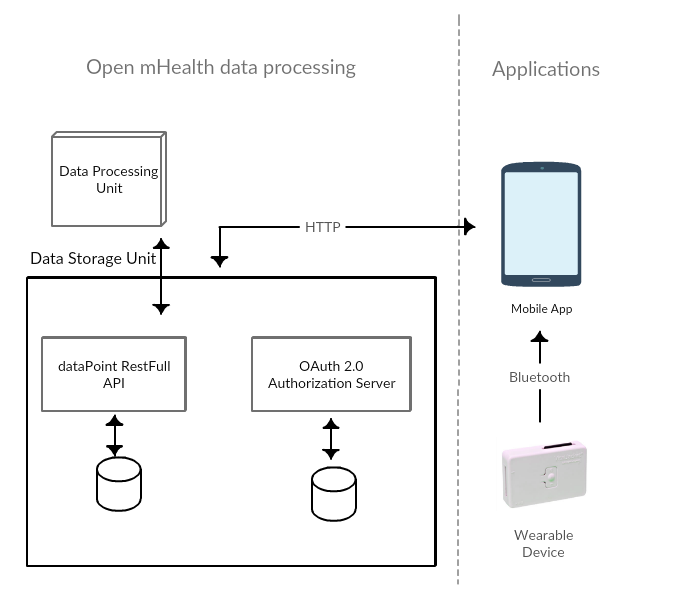
\includegraphics[width=0.9\textwidth]{imgs/omh-arch-exp.png}
  \caption[Arquitetura do caso exploratório com o \textit{Open mHealth}]{Arquitetura do caso exploratório com o \textit{Open mHealth}}
  
  \label{f:exp-omh-arch}
\end{figure}

\subsection{Implementação adicional}
\label{additionalImpl-omh}
Um \textit{dataPoint} é um documento \gls{JSON} composto por um cabeçalho e um \textit{body}, em que o \textit{body} representa um tipo de dados e está em conformidade com o \textit{dataschema} definido no cabeçalho.
No processo de criação de um novo \textit{dataPoint} foi adicionada uma validação, para que fosse garantido que o \textit{body} estava corretamente formatado com o tipo de dados definido no cabeçalho.
Apesar dos \textit{data schemas} especificarem um formato de dados, esta validação não estava a ser efetuada. Esta validação é importante para posteriores consultas e tratamentos dos dados de maneira igual para cada tipo.
\par 


A \gls{OMH} tem definido um conjunto de \textit{data schemas} \cite{omhschemas} que é um conjunto de esquemas de dados criados e disponíveis que especificam um formato de dados para um determinado conteúdo como por exemplo a frequência cardíaca\cite{omhschemas}. Na tabela \ref{t:schemaslist} podemos visualizar alguns dos esquemas de dados existentes. Este conjunto de esquemas de dados pode ser estendido. Ao criar um novo esquema de dados(um novo \textit{data schema}) podemos reutilizar outros já existentes, criando um \textit{data schema} que mesmo não sendo normalizado, utiliza para definição de determinadas propriedades outros \textit{data schemas} normalizados. Para experimentar esta funcionalidade foi então adicionado um novo esquema de dados para que o sistema conseguisse suportar \gls{ECG}. Esta extensão foi conseguida com sucesso e foi uma coisa que saiu um pouco fora do cenário objetivo mas serviu para conseguir perceber melhor a plataforma. \par 
\newpage

\begin{table}[H]
\centering
\label{t:schemaslist}
\begin{tabularx}{1\textwidth}{p{4cm} p{10.7cm}}
 \textbf{Esquema de }  &   \textbf{Nome do ficheiro e Descrição do esquema de dados}  \\
 \textbf{dados (\textit{dataschema})} & \\
\hline
Frequência cardíaca & \textit{heart-rate-1.0.json} \\ 
& Este esquema de dados representa a frequência cardíaca de uma pessoa e a sua relação com a atividade física. O esquema pode ser usado para uma única medição de frequência cardíaca, podendo ser efetuadas várias medições\\ \hline

Relação com a atividade & \textit{temporal-relationship-to-physical-activity-1.0.json} \\
física& Este esquema de dados representa a relação temporal de uma colheita de dados com a atividade física (por exemplo, em repouso, durante o exercício, antes do exercício). \\ \hline

Período de tempo & \textit{time-frame-1.0.json} \\
& Este esquema de dados permite que um período de tempo específico seja definido, como uma hora exata ou um intervalo de tempo. \\ \hline

Pressão arterial & \textit{blood-pressure-2.0.json} \\ 
& Este esquema de dados representa a pressão arterial de uma pessoa como uma combinação da pressão arterial sistólica com a pressão arterial diastólica. Permite indicar se o paciente estava deitado, sentado ou parado quando a medição foi obtida. Este esquema pode ser usado para uma medição única da pressão arterial, podendo ser efetuada várias medições. \\ \hline

Temperatura do corpo & \textit{body-temperature-2.0.json} \\
& Este esquema de dados representa a temperatura corporal e o local do corpo onde foi efetuada a medição. Este esquema pode ser usado para uma medição única, podendo ser efetuadas várias medições. \\ \hline

Glicose no sangue & \textit{blood-glucose-2.0.json} \\ 
& Este esquema de dados representa o nível de glicose no sangue de uma pessoa, e o tipo de amostra do corpo utilizada para efetuar a medição. É ainda apresentada a relação temporal relativamente à refeição e ao sono. Este esquema pode ser usado para uma medição única, podendo ser efetuadas várias medições.
                 
\end{tabularx}
\caption{Tabela com alguns dos esquemas de dados existentes da plataforma \textit{Open mHealth}}
\end{table}



\subsection{Dificuldades e Adaptações}

As dificuldades encontradas não foram muitas, pois a plataforma estava bastante bem estruturada e o grau de complexidade era aceitável. As possíveis falhas desta plataforma era a falta de esquemas de dados para o acelerómetro, \gls{ECG} e para dados demográficos dos utilizadores da plataforma.

\section{Implementação exploratória: FHIR}
%http://hapifhir.io/doc_jpa.html
O \gls{FHIR} ao contrário do \textit{Open mHealth} é apenas uma definição de uma \gls{API} para armazenamento de informação e troca de dados clínicos entre hospitais e clínicas. Esta \gls{API} pode ser desenvolvida de diferentes maneiras. \par 
Existe uma implementação de um projeto de código aberto com o nome \textit{Hapi-FHIR} . Este projeto suporta todos os dados definidos pelo \gls{FHIR} e grande parte das operações sobre eles, como por exemplo criar, editar, eliminar, etc.
\par 
O projeto \textit{Hapi-FHIR} tem um módulo denominado \textit{JPAServer}  \cite{jpa-server}. Este módulo pode ser utilizado para criar um servidor \gls{FHIR}, composto por uma \gls{API} \gls{REST} disponibilizando um conjunto de \textit{endpoints} \gls{HTTP} para que se possa efetuar os pedidos necessários para se guardar os dados no backend. \par

\subsection{Implementação adicional}
O módulo utilizado tinha uma limitação relativa à concessão de autorização sobre os pedidos efetuados, não suportando também a gestão de identidades. Para complementar este módulo foi utilizado o servidor de autorização utilizado também na experiência anterior(o servidor de autorização do \gls{DSU} do \textit{Open mHealth}).
No \textit{JPAServer} foi então desenvolvido um Intercetor que o que fazia, era verificar se o pedido efetuado era acompanhado por um \textit{token} de acesso, caso isso acontecesse a validade do \textit{token} era verificada pelo servidor de autorização e então em caso de sucesso era fornecido o acesso ao pedido solicitado. Na figura \ref{f:exp-fhir-arch} temos então a arquitetura final deste caso exploratório.
\begin{figure}[H]
  \centering
  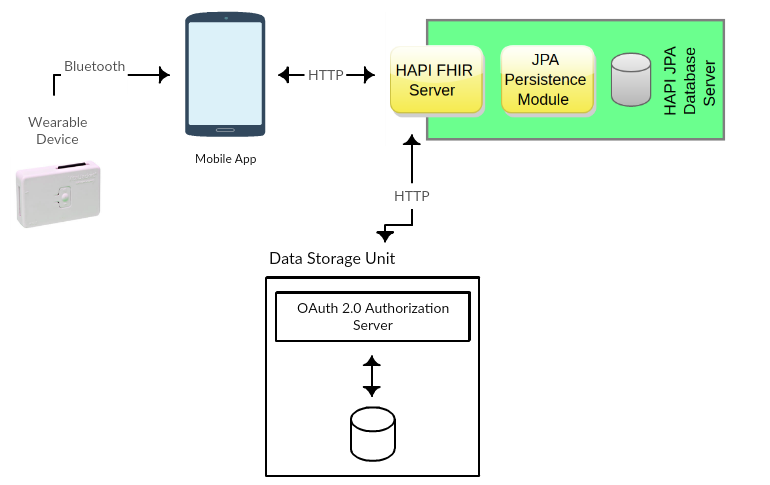
\includegraphics[width=0.9\textwidth]{imgs/fhir-arch-exp.png}
  \caption[Arquitetura do caso exploratório com o FHIR]{Arquitetura do caso exploratório com o FHIR (Adaptado de)\cite{hapi-index}}
  
  \label{f:exp-fhir-arch}
\end{figure}

\subsection{Dificuldades e Adaptações}
As dificuldades encontradas ainda foram algumas, neste caso temos uma definição de uma \gls{API} em vez de uma plataforma em si, ou seja, foram encontradas várias supostas resoluções, e no caso do \textit{Hapi-FHIR} estava dividida por vários módulos, que por um lado até se pode tornar mais vantajoso porque acabamos por utilizar só aquilo que é necessário. As possíveis falhas desta \gls{API} era a falta de tipos de recursos para o acelerómetro e \gls{ECG}. Ainda temos a falta de um servidor de gestão de identidades e a concessão de autorização ao pedidos efetuados.

\section{Implementação exploratória: \textit{Google Fit}}
%https://developers.google.com/fit/rest/

O \textit{Google Fit} disponibiliza uma \gls{API} \gls{REST} que permite o armazenamento de dados na nuvem. Esta \gls{API} permite a criação  de \textit{datasources}. Um \textit{datasource} é criado por cada utilizador e representa  um conjunto de dados de um determinado tipo. Relativamente à concessão de acesso aos serviços \gls{REST} é utilizado o serviço de autenticação e autorização da Google baseado em OAuth 2.0. 
\par
O cenário objetivo foi desenvolvido com sucesso e na figura \ref{f:exp-googlefit-arch} podemos ver a arquitetura final deste caso exploratório.
\begin{figure}[H]
  \centering
  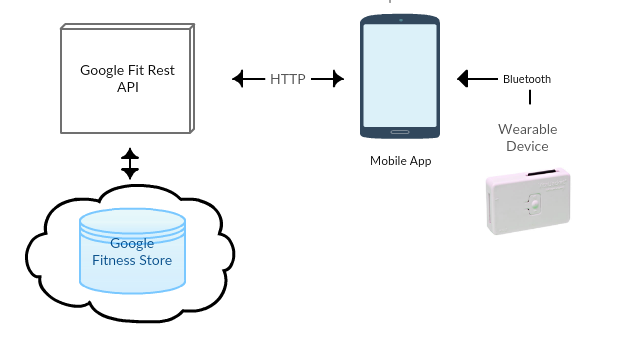
\includegraphics[width=0.9\textwidth]{imgs/googlefit-arch-exp.png}
  \caption[Arquitetura do caso exploratório com o \textit{Google Fit}]{Arquitetura do caso exploratório com o \textit{Google Fit}}
  
  \label{f:exp-googlefit-arch}
\end{figure}

\subsection{Dificuldades e Adaptações}

Um dos problemas encontrados nesta fase de exploração é que apesar do tipo de dados poder ser extensível, apenas era aceite dados do tipo inteiro e \textit{float}, ou seja, não são suportados propriedades do tipo objeto ou vetor. Esta \gls{API} não tinha suporte para dados do tipo \gls{ECG}, acelerómetro e dados demográficos.

\section{Resultados e lições aprendidas}
%ico: sistematizar aquilo que foi possível concluir das implementações exploratórias discutir pontos forte / fracos observados

\textbf{\textit{Google Fit}}
\par
Esta plataforma tem como um ponto muito positivo utilizar o serviço de autenticação e autorização da Google e o facto dos dados ficarem armazenados na nuvem.\par 
O primeiro ponto negativo a apontar é relativo à extensibilidade dos dados, só permitir dados do tipo inteiro e \textit{float}. Para exemplificar como isto pode vir a ser um problema, no caso do \gls{ECG}, por segundo o sensor envia 500 valores, para que se possa formar um \gls{ECG} com alguma precisão, como esta plataforma não suporta vetores, tinha que ser feito 500 pedidos ao servidor por segundo para conseguir guardar e posteriormente visualizar um \gls{ECG} fidedigno. Um outro ponto negativo é o fato de esta plataforma ser da Google, o que isto quer dizer é que não é possível correr a plataforma de forma nativa e efetuar implementações extra sobre as já existentes.
\par
\textbf{\textit{Open mHealth}}
\par
Como o \gls{OMH} é um projeto de código aberto um grande ponto forte é a possibilidade da implementação de novas funcionalidades poder ser efetuada com mais facilidade, como por exemplo a adição da validação dos dados inseridos. Tendo em conta que o projeto foi desenvolvido com o intuito de diminuir a ocorrência de formatos de dados próprios por cada aplicação móvel no âmbito da saúde, esta pode muito bem ser uma solução para o \textit{backend} do produto proposto, dado que a possibilidade da extensibilidade dos dados também é possível através da criação de novos \textit{data schemas} que são posteriormente utilizados para ser efetuada a validação dos dados inseridos.
\par
O conjunto de esquemas de dados criados para dar suporte à plataforma da \gls{OMH} foi criado utilizando referências de dados normalizados no ambiente hospitalar e clínico, uma dessas referências utilizada foi a \gls{API} do \gls{FHIR}.
\par
\textbf{FHIR}
\par
Um dos pontos fracos do FHIR neste caso em concreto do \textit{Hapi-FHIR} é a falta de serviço de autenticação e autorização. Um outro ponto fraco é a inexistência de um projeto de código aberto ''oficial'', ou seja, existe bastantes possibilidades diferentes e descobrir qual poderia utilizar e da melhor maneira não foi uma coisa fácil.
\par
Um dos pontos fortes é saber que esta definição da \gls{API} é bastante utilizada por hospitais e clínicas.
\par
\textbf{Análise Comparativa}
\par
Tendo em conta que o produto proposto tinha como um dos objetivos guardar dados relativos ao \gls{ECG}, o \textit{Google Fit} é limitado relativamente ao tipo de dados, ou seja, não suporta vetores para guardar os dados, ficando logo praticamente excluído como possível escolha para o \textit{backend}.
Ficamos agora então com o \textit{Open mHealth} e o \gls{FHIR}, nenhum deles está apto na totalidade para ser utilizado sem qualquer alteração. Por um lado temos falhas nas duas plataformas que não contemplam todos os tipos de dados que precisam de ser guardados, como por exemplo o acelerómetro e o \gls{ECG}, apesar do \gls{FHIR} estar mais completo neste assunto.
Para além disto o \gls{FHIR} não contém nenhum serviço de autenticação e autorização sendo necessário utilizar um serviço externo.
Não podemos dizer que o \gls{FHIR} não servia como solução, mas tendo em conta que nenhum deles é perfeito, e que o \textit{Open mHealth} é um projeto que foi desenvolvido com o objetivo de uniformizar os \textit{backends} na área das aplicações móveis na área de saúde, vamos optar pela utilização desta plataforma, dando uma oportunidade a um projeto inovador, com o intuito também de perceber se mais tarde, pode ou não vir a ser utilizado em diferentes projetos como \textit{backend} de aplicações móveis na área da saúde, ou até em projetos de \gls{ID}.

\cleardoublepage